\documentclass[headings=standardclasses,parskip=half]{scrartcl}

\usepackage[french]{babel}
\usepackage[margin=3cm]{geometry}
\usepackage{graphicx}
\usepackage[hidelinks]{hyperref}

\titlehead{
    \begin{center}
        
\includegraphics[width=5cm]{n7.png}
    \end{center}
}
\subject{Projet Données Réparties}
\title{Rapport}
\subtitle{}
\author{Enzo PETIT \and Nam VU}
\date{16 janvier 2022}
\publishers{ENSEEIHT – 2SN-A}


\begin{document}

\maketitle

\newpage

\tableofcontents

\newpage

\section{Introduction}

Le projet Linda a pour but de réaliser un espace partagé de données
typées.

Une version à mémoire partagée avec gestion de callback a été réalisée
ainsi qu'une version client-serveur en RMI se reposant sur cette dernière.

Pour la première version, la classe \texttt{linda.shm.CentralizedLinda}
a ainsi été complétée et des tests unitaires sous
\href{https://junit.org/junit5/}{JUnit 5}
ont été rédigés dans \texttt{linda.test.CentralizedLindaTest}.

La version client-serveur se trouve quand à elle dans le package
\texttt{linda.server} et utilise la version \textit{shm} inchangée pour
la partie serveur.

Enfin quelques applications utilisant Linda ont été réalisées
telle que la recherche de nombre premiers selon l'algorithme du
crible d'Erathosthène, en séquentiel et parallèle, ainsi que la
parallèlisation de l'application de recherche.

\section{Version en mémoire partagée}

\textit{Cette section reprend le rapport provisoire de décembre dernier.}

\subsection{Réalisation}

A l'instanciation, \texttt{CentralizedLinda} initialise trois tableaux
pour le stockage des tuples (\texttt{tupleSpace}) et les events
\emph{take} (\texttt{takeEvents}) et \emph{read} (\texttt{readEvents}).

Ces tableaux sont de type \texttt{CopyOnWriteArrayList} qui est une
variante \emph{thread-safe} de l'\texttt{ArrayList} classique adaptée
à un contexte concurrent où le nombre de lectures est bien supérieure
au nombre d'écritures.

Suivent après les détails d'implémentation des différentes opérations,
plus ou moins dans l'ordre de réalisation :

\subsubsection{\texttt{tryTake}, \texttt{tryRead}}

Ces deux méthodes sont non bloquantes, on itère simplement sur la liste
(en partant de la tête) et on renvoie le premier tuple (le plus vieux)
qui match le template. \texttt{null} est renvoyé si aucun tuple
actuellement stocké ne correspond.

\subsubsection{\texttt{takeAll}, \texttt{readAll}}

Même chose que précedemment mais on stocke tous les tuples correspondants
dans une \texttt{ArrayList} que l'on renvoie à la fin (qui est vide
si aucun résultat).

\subsubsection{\texttt{eventRegister}}

En commençant à vouloir implémenter les \texttt{take} et \texttt{read}
bloquant on s'est demandé comment pouvait-on "proprement" et avec le
moins d'effort possible bloquer et débloquer les appels : le principe
des event nous a paru bien adapté pour réaliser cette tâche
(détails plus loin).

En mode \texttt{IMMEDIATE} un tuple est retourné immédiatement dans
le callback en cas de match sur l'espace actuel
(via \texttt{tryTake}/\texttt{tryRead}),
sinon on range l'event en attente dans le tableau correspondant
(\texttt{takeEvents} ou \texttt{readEvents}).

Le callback est transformé en amont en \texttt{AsynchronousCallback}
afin d'éviter les problèmes liés au blocage du thread principal ou
d'enregistrements récursifs de callbacks.

\subsubsection{\texttt{write}}

La méthode \texttt{write} étant la "porte d'entrée" de tous les tuples
vers l'espace de stockage de Linda, c'est là qu'on en profite pour
"résoudre" les event en attente le cas échéant.

Ainsi on itère d'abord sur les \emph{read} en attente (\texttt{readEvents}),
vérifie si le tuple à écrire "match" le template de l'event et le cas
échéant on appelle le callback correspondant.

Ensuite on fait de même avec les \emph{take} en attente (\texttt{takeEvents})
mais au premier match (du plus vieux), on résout le callback et on retourne,
immédiatement. Le tuple n'est pas enregistré et les \emph{take} en attente
dessus mais plus récents attendront le prochain tuple correspondant.

Finalement si aucun \emph{take} n'attendait le tuple, on le sauvegarde dans
\texttt{tupleSpace}.

Un tuple en entrée peut ainsi résoudre tous les \emph{read} en attente mais
qu'un seul \emph{take} en attente, le plus vieux.

\subsubsection{\texttt{take}, \texttt{read}}

Un \emph{take} ou \emph{read} bloquant revient à enregistrer un event
\emph{immédiat} dont le callback renvoie le tuple passé en entrée,
rester bloqué jusqu'à résolution de celui-ci et finalement renvoyer
son résultat.

On utilise pour faire ça une \texttt{LinkedBlockingQueue}, queue bloquante :
le callback de l'event correspond à la méthode \texttt{offer} de la queue
(dépôt non bloquant) qui sera éventuellement appelée lors d'un \emph{write}.

Le \texttt{take}/\texttt{read} reste lui bloqué sur le \texttt{take} de la
queue et renverra son résultat quand il sera débloqué par un dépôt dans
la queue.

\subsection{Tests}

Tous les tests \texttt{Basic} fournis passent en l'état.

Une classe de tests unitaires \href{https://junit.org/junit5/}{JUnit 5}
\texttt{linda.test.CentralizedLindaTest} a aussi été écrite.

\begin{figure}[h]
    \centering
    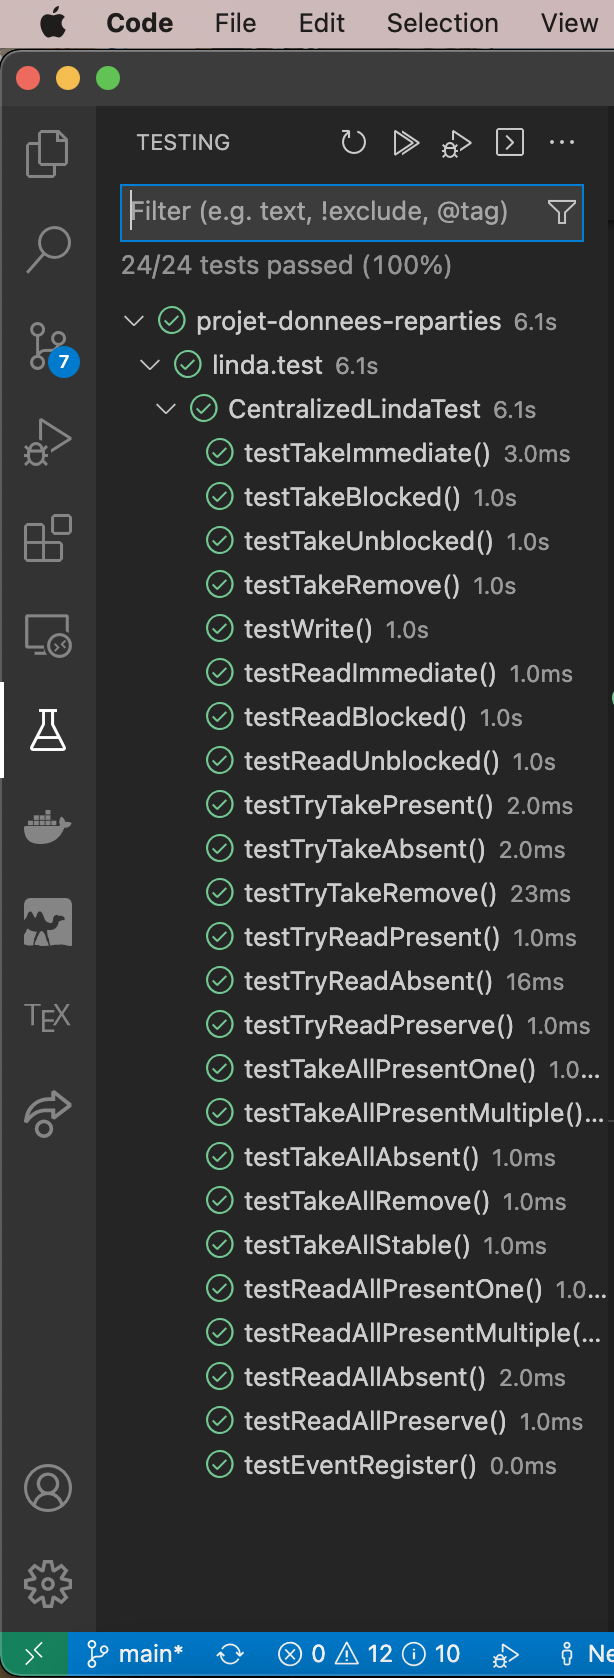
\includegraphics[scale=0.5]{tests-results.png}
    \caption{Résultats des tests définis dans
        \texttt{linda.test.CentralizedLindaTest}\\
        (Visual Studio Code + Extension Pack for Java)}
\end{figure}

\section{Version client / mono-serveur}

\subsection{Serveur}

Une interface \texttt{LindaServer} a été définie, étandant \texttt{Remote},
et reprend les méthodes définies dans l'interface \texttt{Linda} à la
différence que toutes les méthodes \texttt{throws RemoteException} et
que \texttt{eventRegister} prend en paramètre un \texttt{eventRegister}.

\texttt{eventRegister} est une interface qui étand aussi \texttt{Remote}
et représente un callback à exécuter sur le client.

L'implémentation de \texttt{LindaServer} est rédigée dans
\texttt{LindaServerImpl}. Cette classe initialise un noyau Linda en
mémoire partagée et transmets directement tous les appels distants au
noyau à l'exception du \texttt{eventRegister} : pour cette méthode,
on transmet au kernel un callback local qui résoudra le callback distant.
Ainsi tout est transparant pour le noyau en mémoire partagée.

\subsection{Client}

De la même manière \texttt{LindaClient} récupère un \texttt{LindaServer}
en RMI puis fonctionne de manière transparente pour les appplications en
local en ne faisant que transferer directement toutes les requêtes au
serveur distant.

Exception est encore faite pour \texttt{eventRegister} qui est un peu plus
complexe: on envoie au serveur un \texttt{RemoteCallback} via
\texttt{RemoteCallbackAdapter} qui s'occupera de répondre au callback
local côté client.

\section{Applications}

\subsection{Calcul des nombres premiers}

\subsection{Recherche approximative dans un fichier}

\section{Conclusion}

\end{document}
